{\chapter{Analyse}}
\label{sec:analyse}
Zusätzlich zu den maschinellen Lernkomponenten stellt Unity auch Demonstrationsumgebungen bereit, in denen verschiedene Lösungen für gängige Verstärkungslernprobleme implementiert sind. In der Walker-Demo wird ein physisch simulierter Charakter darauf trainiert, zu einem Zielwürfel zu laufen. Diese Demo-Umgebung implementiert bereits einige Grundlagen für die Steuerung eines physisch simulierten Charakters. Aus diesem Grund wird in dieser Arbeit die Walker-Demo als Basis für die Entwicklung genutzt. In diesem Kapitel wird daher die Walker-Demo analysiert, um in den folgenden Kapiteln darauf aufzubauen.

\section{Szenenaufbau}
Die Szene besteht aus einem quadratischen Spielfeld mit Boden und Wänden die der Charakter nicht verlassen kann (siehe Abbildung \ref{fig:walker_aufbau}). Der Läufer startet jede Trainingsepisode in der Mitte des Spielfelds. Das Ziel wird zu beginn zufällig platziert. Bei jedem erreichen des Ziels wird die Zielposition erneut zufällig bestimmt.

\begin{figure}[H]
  \centering  
  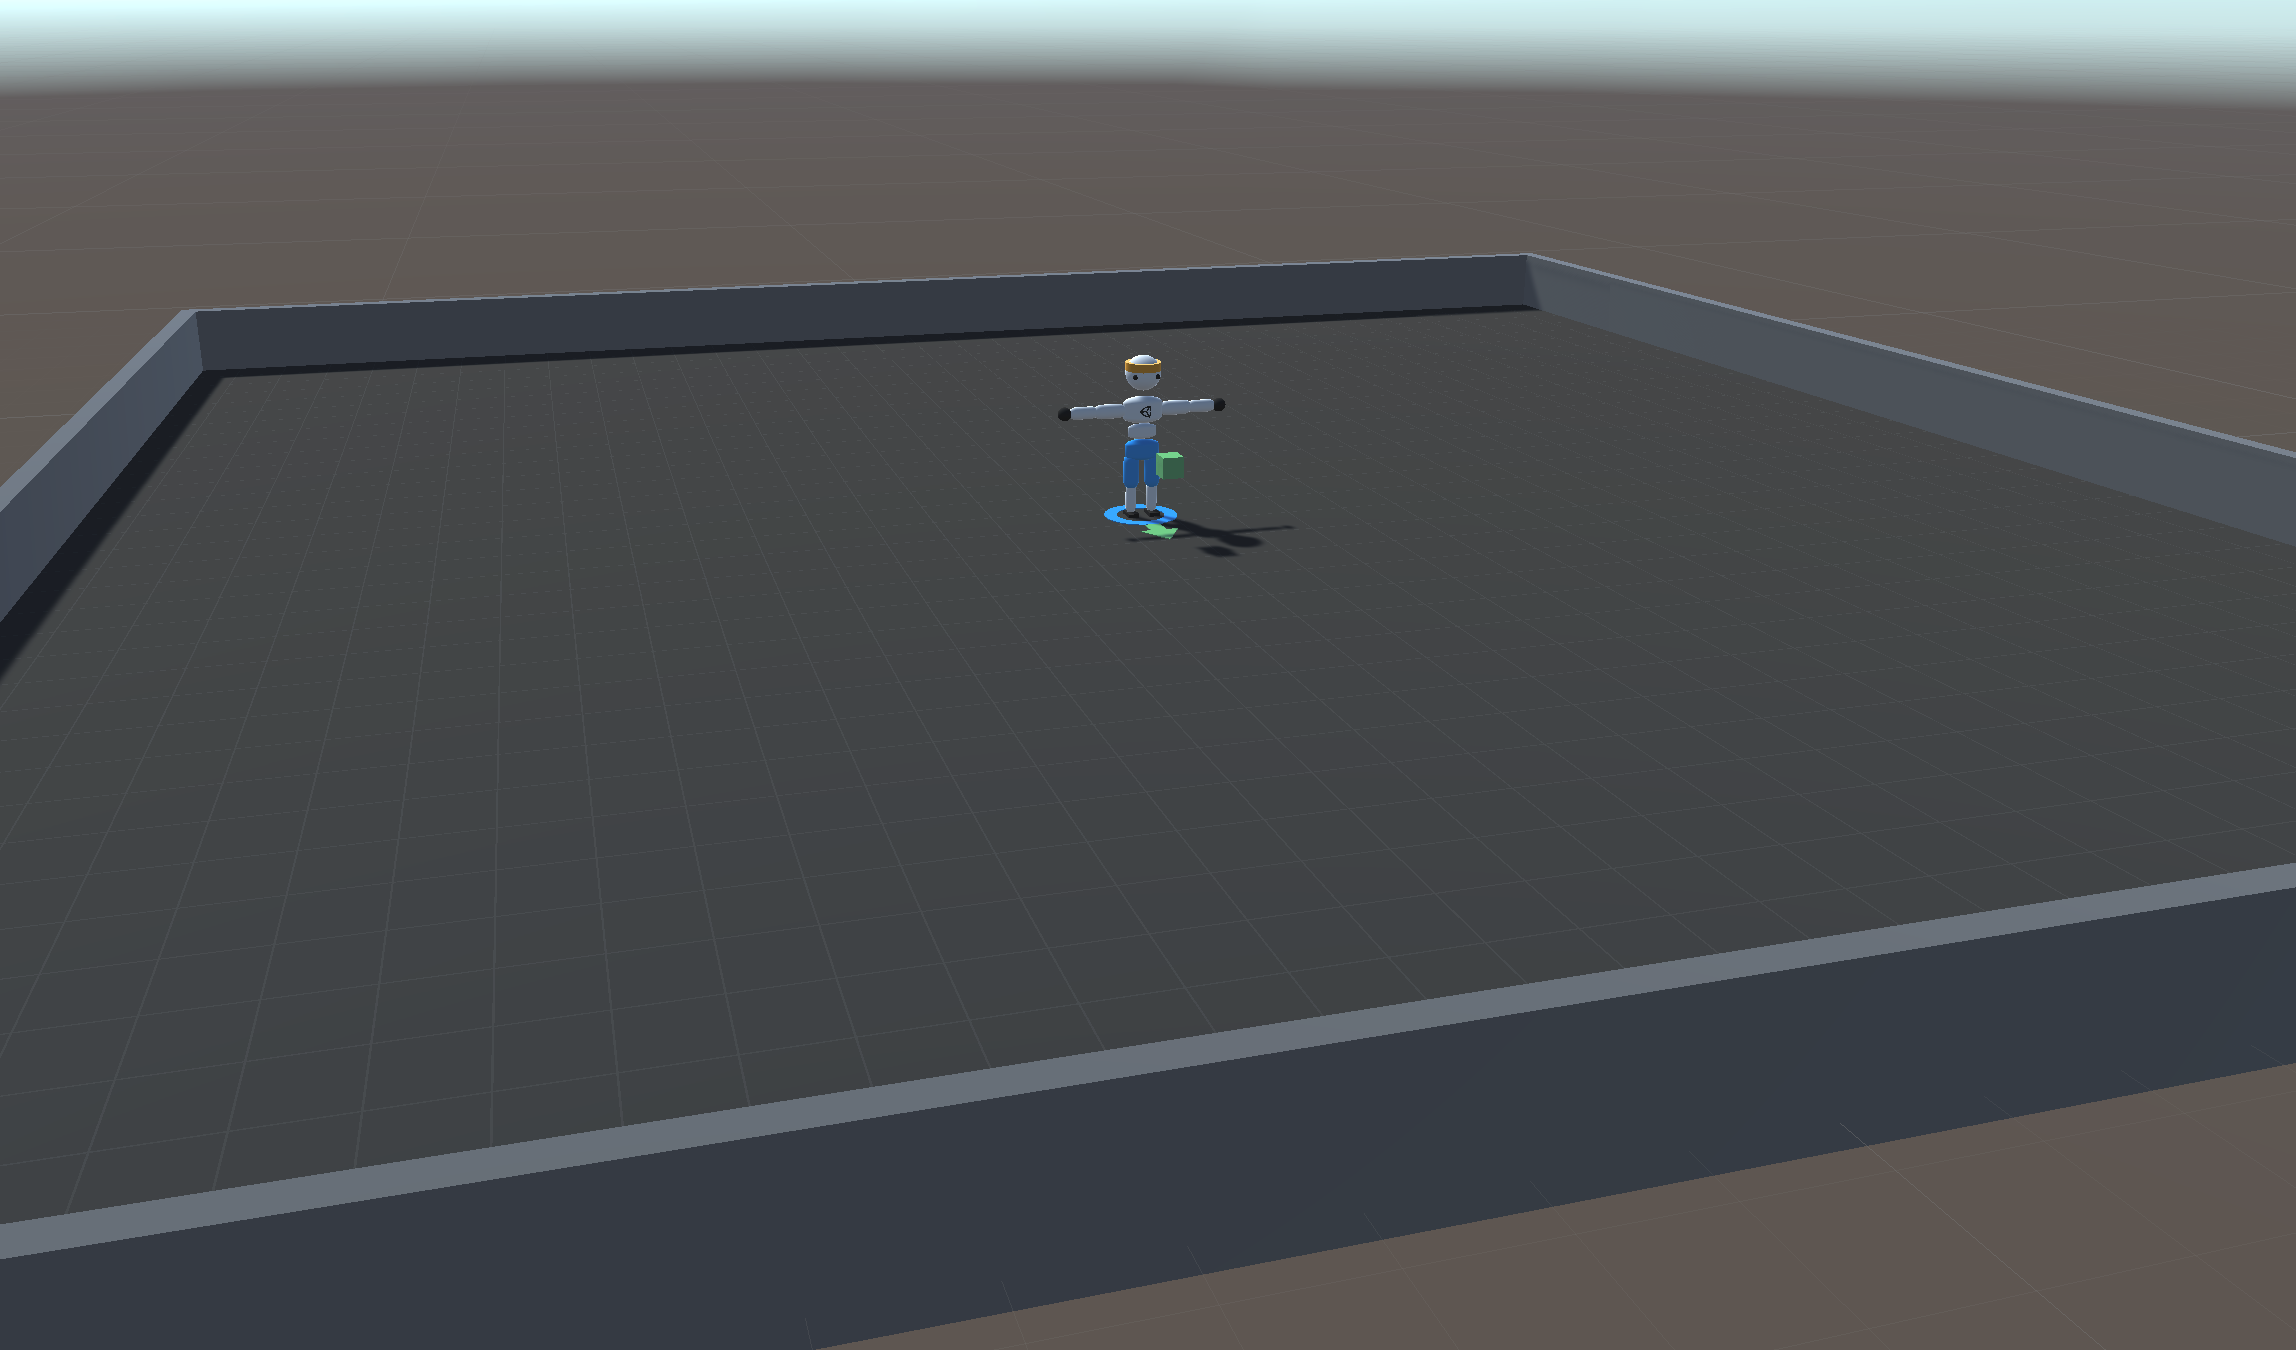
\includegraphics[scale=0.35]{img/walker_aufbau.png}
  \caption{Walker-Demo Szenenaufbau}
  \label{fig:walker_aufbau}
\end{figure}

\section{Physikkomponenten und -konfiguration}
Der Körper besteht aus 11 Kapseln, drei Kugeln und 2 Quadern, jeder dieser Formen hat eine Festkörper und eine Kollisions Physikkomponente. Zwischen den Körperteilen werden die Gelenke als Kugelgelenke simuliert. Die genaue Physikkonfiguration der Körperteile werden veranschaulicht in Tabelle \ref{table:walker_körperteile}

\begin{table}[H]
  \centering
  {\rowcolors{2}{lightgray}{gray!50!lightgray!50}
  \begin{tabular}{ |p{3cm}|p{3cm}|p{2cm}|p{4cm}|p{2cm}| }
  \hline
  Körperteil& Verbundenes Körperteil & Gewicht & Winkellimits & Form \\
  \hline
  Hüfte & - & 15kg & - & Kapsel \\
  Wirbelsäule & Hüfte & 10kg & x(-20,20) y(-20,20) z(-15,15) & Kapsel \\
  Oberkörper & Wirbelsäule & 8kg & x(-20,20) y(-20,20) z(-15,15) & Kapsel \\
  Kopf & Oberkörper & 6kg & x(-30,10) y(-20,20) & Kugel \\
  Oberarm LR & Oberkörper & je 4kg & x(-60,120) y(-100,100) & Kapsel \\
  Unterarm LR & Oberarm & je 3kg & x(0,160) & Kapsel \\
  Hand LR & Unterarm & je 2kg & - & Kugel \\
  Oberschenkel LR & Hüfte & je 14kg& x(-90,60) y(-40,40) & Kapsel \\
  Unterschenkel LR & Oberschenkel & je 7kg &  x(0,120) & Kapsel \\
  Fuß LR & Unterschenkel & je 5kg & x(-20,20 y(-20,20) z(-20,20) & Quader \\
  \hline
  \end{tabular}}
  \caption{Walker Agent Körperteile}
  \label{table:walker_körperteile}
\end{table}

\section{Agent implementierung}
In diesem Kapitel wird die Agenten Implementierung näher Analysiert.
\begin{figure}[H]
  \centering  
  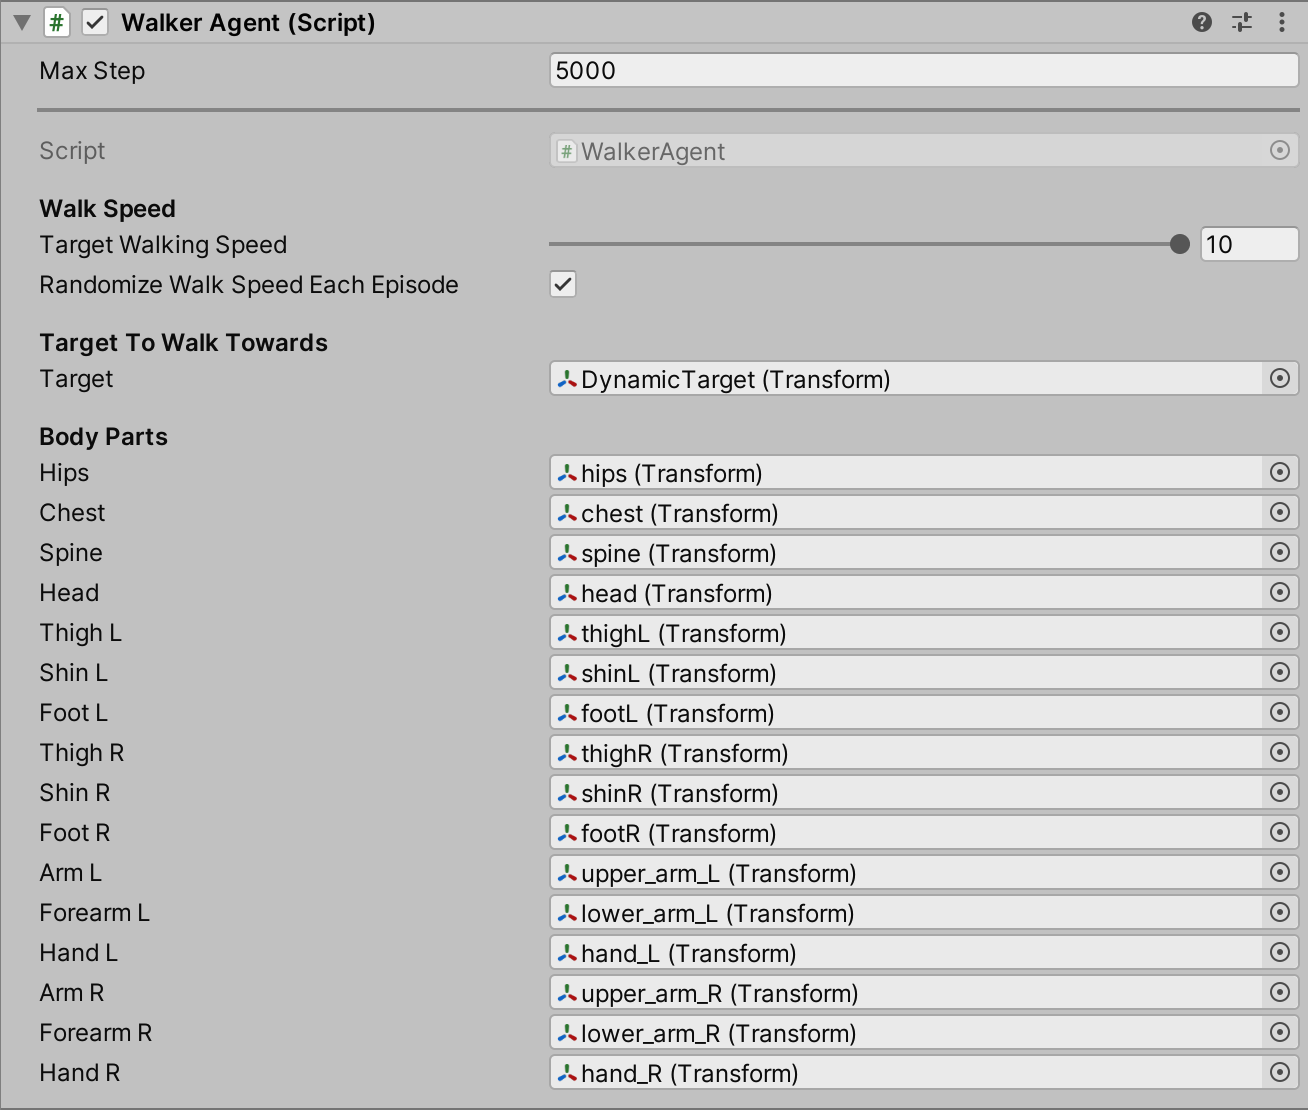
\includegraphics[scale=0.5]{img/agent_konfiguration.png}
  \caption{Agent Konfiguration}
  \label{fig:agent_konfiguration}
\end{figure}

Abbildung \ref{fig:agent_konfiguration} zeigt die Agentenkomponente im Inspektor. Um die Komponente zu nutzen müssen hier die Körperteile des Walkers referenziert werden. Zusätzlich kann eine Zielgeschwindigkeit festgelegt werden und ob die Geschwindigkeit variieren soll während dem Training. Als letztes muss auch das Zielobjekt referenziert werden.

$Q_{Hüfte}=Quaternion(\vec{Hüftrichtung} - \vec{Zielrichtung})$\\
$Q_{Blick}=Quaternion(\vec{Blickrichtung} - \vec{Zielrichtung})$

$S=\{
\\|\vec{Zielgeschwindigkeit} - \vec{Durchschnittsgeschwindigkeit}|,
\\\vec{Durchschnittsgeschwindigkeit},
\\\vec{Zielgeschwindigkeit},
\\Q_{Hüfte},
\\Q_{Blick},
\\\vec{Zielposition},
\\K_1,K_2,...,K_n
\\\}$

$K=\{
\\Bodenkontakt,
\\\vec{Geschwindigkeit},
\\\vec{Rotationsgeschwindigkeit},
\\\vec{Position} - \vec{Hüftposition}.
\\Quaternion(Lokale Rotation),
\\Gelenkstärke
\\\}$

$A=\{
\\Rotationswinkel_1, Rotationswinkel_2,...,Rotationswinkel_n,
\\Gelenkstärke_1, Gelenkstärke_2,...,Gelenkstärke_n
\\\}$

$V_\delta=Clip(|\vec{Geschwindigkeit} - \vec{Zielgeschwindigkeit}|, 0, |\vec{Zielgeschwindigkeit}|)$ \\
$R_V=(1 - (V_\delta / |\vec{Zielgeschwindigkeit}|)^2)^2$ \\
$R_L=(\vec{Zielrichtung} \cdot \vec{Blickrichtung})+ 1) \cdot 0.5$ \\
$R=R_V \cdot R_L$

Initialisierung bzw Episodereset erklären
Orientation Object erklären
Zielsetzung erklären
Rewardfrequenz erwähnen